\section{Objectives and Activities}

The project targets the evaluation of the scalability of the two kinds of compositions explained above. To make this assessment, we first needed a composition to evaluate. Thus we designed a synthetical orchestration in witch each partner is another synthetical orchestration, recursively, the second's partners are also orchestrated services, until the last specific composition. The topology generated from this design is a tree, each node (first kind of orchestrated service) has a pre-defined number of children. The depth of the tree is also predefined. The message received in the root node is propagated, in a sequential way, through its children until it reaches the leaf node (the second kind of service on the process). When the leaf node receives the message, it sends the message back to its sender, that sends the message back until it arrives at the root, which replies to the client. A simple example with 3 children per node and depth of 2 is shown in Figure \ref{synthetical-example}.

\begin{figure}[htb]
	\centering
	\includegraphics[width=\textwidth]{images/synthetical-example}
	\caption{Example of a composition with 3 children per node and depth of 2. With its flow of messages}
	\label{synthetical-example}
\end{figure}

This tree is a choreography of orchestrated services: each node and its children are the orchestration and the entire process is a choreography.

\subsection{Composition Generator}
To generate the tree structure described above, at first we developed ``hardcoded'' orchestrations using \emph{Eclipse with BPEL Designer plugin}, but it alone could not execute the modeled process. Then we began a search of engines for orchestrations. One big requirement for the tools we were going to use was that they should be Open Source, GPL or LGPL, so that they could meet the required licenses of Baile and CHOReOS projects (GPL), the first service engine we came across was \emph{Apache's ODE}. At first glance it worked well, but it could not compile the Eclipse generated processes and it is licensed under Apache License, incompatible with ours.

As ODE could not compile the generated orchestrations, we were forced to look at the code generated for debugging, and we did not appreciate that horrible code. That was the time to look for another development tool and another engine as well. We found \emph{NetBeans Enterprise Edition version 6.5} that was known for its good usage and intuitive Graphical User Interface (GUI). We redesigned the web service orchestrations in NetBeans, the re-work was indeed easy to do and the generated code was human readable. The search for an engine was a little more complicated, and NetBeans was able to execute its orchestrations. So we postponed the search for an engine in order to develop the synthetical orchestrations.

The development of the Ruby script to generate synthetical orchestrations began using TDD, but in this specific case, the test code had literal strings exactly as the tested code did. This similarity put in doubt if TDD was really helping the development or not. This kind of discussion is not in this project scope, we have just decided not to use this technic at this time. When the development phase was over, we discovered that TDD \emph{could} have helped us to find bugs and give us more confidence to make big refactorings.

When ready, the generator was able to create orchestrations that were executable within Netbeans, the script generated the composition tree and also, for each node of the tree, a set of WSDL and BPEL files corresponding to the service of that node. Then we started the study of Amazon EC2 and the improvement of the Ruby script to instantiate virtual machines on EC2 for each node o the tree. At this moment the code was starting to get ugly. It was time for refactoring.

One big discovery we made at that time was that NetBeans could not execute the orchestrations from a command-line shell, it required a GUI for the execution process, which made its use no longer feasible anymore due the fact that the only interface with Amazon EC2 instances is through \emph{ssh}. We had to get back to the search of an orchestration engine. Meanwhile the generator was instantiating all the machines we would needed for the composition's deployment, but we also discovered that we had a quota in Amazon that limited us to use only 20 instances at a time.

Orchestra was the next tested engine. Even though it had good comments about it, we could not execute any orchestration in it. With the lack of documentation and support, the development was fully stagnant until we could find a usable engine. After a couple of weeks searching in forums and papers, the solution came from the CHOReOS project new orders. They demanded that the project used PEtALS ESB, what was great for us. Not only were we unable to find any good open source engine --- and the only we knew that worked, Apache's ODE, had an incompatible license --- but also PEtALS ESB had the simplest install and setup process among all the servers studied; this was the most essential feature to build the automated process. We started the experiments on the standalone mode of PEtALS, which is an ESB with just one node.

PEtALS executed the generated orchestrations seamlessly on the standalone version. We were back to the development of the generator and deployer for Amazon EC2. After some adjusts, the generator was creating the tree, instantiating virtual machines on Amazon EC2, creating the compositions, configuring each instance to become a node of the PEtALS Bus, starting the PEtALS server in each node, and deploying the services on the ESB. This whole process is parallelized for each node, and the steps of the process can be followed in the shell's standard output, as shown in Figure \ref{generation-output}.

\begin{figure}[htb]
	\centering
	\includegraphics[trim= 10mm 0mm 10mm 0mm, clip, width=\textwidth]{images/generation-output}
	\caption{Example output from running the generator script for a tree with depth of 1 and 10 children per node}
	\label{generation-output}
\end{figure}

When it is finished, the generator outputs the host of the process (\emph{Public DNS} of Root Node), from which port it is reachable, the path to the service, and the ID of this root node (to compose the SOAP messages).

Although all the phases have been completed, the connection from outside to the cloud was very unstable and unpredictable. This issue is probably the source of the problem: when sending a message to the composition instantiated on the cloud, it returns a SOAP fault. We contacted the developers of PEtALS for some help, and turns out that they do not know how to solve the issue for now, they asked to use another PEtALS tool to monitor the process, but we encountered another bug on this new tool. This discussion with the developers is still happening while the present moment of this document written. To be able to make at least more complex tests, we started using a LAN (called ``Revoada'') inside the IME-USP.

The tests proceeded in a smaller scale in ``Revoada'', since it has eight computers in LAN, instead of the twenty possibles virtual machines from Amazon EC2. But we came up with some interests results, explained on the next Section.


\subsection{Message Sender}

To evaluate the responses of the synthetical compositions, we developed another Ruby script to send messages of sizes $s$ and with a frequency of $f$ messages per second.

Given the fact that the connection with the composition may alter the results, we added a third parameter to define how many times the batch of messages would be sent, so when there is a lot of traffic on the network, any outlier will not be representative on the overall average. During the execution, the script shows four numbers for each batch of messages sent, they represent (in order of appearance):

\begin{itemize} 
	\item \textbf{user} is the time spent (in seconds) with the execution of actions of the script, for example calling a class method
	\item \textbf{system} is the time spent (in seconds) with system calls, for example creating a \emph{fork}
	\item \textbf{total} is the sum of \emph{user} and \emph{system} times
	\item \textbf{real} is how long it passed (in seconds) since the task begin until its end
\end{itemize}

An example of its execution is shown in Figure \ref{send-msg-output}.

\begin{figure}[htb]
	\centering
	\includegraphics[width=0.8\textwidth]{images/send-msg-output}
	\caption{Example output from running the send message script with $S = 1$, $F = 1$, $BatchSize = 10$}
	\label{send-msg-output}
\end{figure}

To minimize the latency problem, we ran the \textunderscore{``send\_messages''} script on one of the machines of the LAN.